% ============================================================================
% npj Computational Materials -- Article
% Constraints (Guide to Authors, checked 2026-08-28; re-check before submission):
%   abstract <= 250 words, unstructured | main text <= 5,000 words
%   <= 6 tables+figures combined (currently 6 figures + 2 tables = 8, OVER:
%     Fig. 6 and Table 2, the interface chemistry, are in the main text for
%     this draft and must move to the SI (Fig. S1 / Table S2) before submission)
%   <= ~50 references, numerical superscript citations only
%   section order fixed: Title -> Abstract -> Intro -> Results -> Discussion ->
%     Methods -> Acknowledgements -> Competing Interests -> Contributions ->
%     Funding -> References -> Figure legends -> Tables -> Figures
%   code availability BEFORE data availability, both at end of Methods
%   INITIAL SUBMISSION (live guide, checked 2026-09-25): format-free; a single
%     compiled PDF with figures inline, each legend on the same page as its
%     figure. LaTeX source only at acceptance.
%   AT ACCEPTANCE: legends move to a Figure Legends section after References,
%     figures/tables upload as separate files, paste .bbl for thebibliography
%
% Rebuild 2026-09-25 from commit f08c71a (3 ns diffusion stage). Lines tagged "% VERIFY" carry a
% statement taken from the 2026 BS thesis or inferred from file names; check
% against the current pipeline before submission. Material moved out of the
% main text lives in si_v0.tex (Supplementary Notes 1-7).
% ============================================================================

\documentclass[11pt]{article}

\usepackage[utf8]{inputenc}
\usepackage[T1]{fontenc}
\usepackage{amsmath,amssymb}
\usepackage{graphicx}
\usepackage{booktabs}
\usepackage[super,comma,sort&compress]{natbib}
\usepackage[left]{lineno}
\usepackage{setspace}
\doublespacing
\usepackage[margin=1in]{geometry}

\linenumbers
\newcommand{\figslot}[2]{%
  \IfFileExists{#1}{\includegraphics[width=0.85\linewidth]{#1}}%
  {\fbox{\parbox[c][4cm][c]{0.8\linewidth}{\centering\small #2}}}}

\begin{document}

% ---------------------------------------------------------------------------
% TITLE PAGE
% ---------------------------------------------------------------------------
\title{Latent-space-driven active learning with DFT-FE for solid-state battery
interfaces: application to Li-metal/LLZO}

% Running title (<=50 letters and spaces):
% Active learning for solid-state battery interfaces

\author{
Mehul Darak$^{1}$ \and
Rajdeep Boral$^{2}$ \and
Kartick Ramakrishnan$^{1}$ \and
Phani Motamarri$^{1}$ \and
G.~P.~Das$^{2}$
}
\date{}
\maketitle

\noindent
$^{1}$Indian Institute of Science, Bangalore, India \\
$^{2}$TCG CREST, Kolkata, India \\
% [TODO] mark the corresponding author with $^{\ast}$ and give the email here.

\vspace{1em}

% ---------------------------------------------------------------------------
% ABSTRACT (<=250 words)
% ---------------------------------------------------------------------------
\section*{Abstract}
Solid-state batteries are limited at their internal interfaces, and resolving
interfacial chemistry requires molecular dynamics on cells of hundreds to
thousands of atoms, the domain of machine-learned interatomic potentials. Two
compromises usually enter such potentials. Their reference data come from cells
that lack the free-surface environments an interface contains, and plane-wave
density functional theory represents a surface only through a sandwich with a
second interface or a vacuum-padded, dipole-corrected slab whose cost grows with
the vacuum. We present a pipeline that removes both. Reference labels come from
DFT-FE, a real-space finite-element Kohn--Sham code whose mixed boundary
conditions leave the surface normal genuinely open, at the 420--1378-atom scale
on which the potential is deployed; training structures are acquired by
farthest-point sampling in a pretrained MACE model's own latent space, stopping
when the candidate pool is covered. Applied to the
Li-metal/Li$_7$La$_3$Zr$_2$O$_{12}$ interface over six iterations,
component-wise force error falls from 121 to 72~meV/\AA\ (RMSE) and from 70 to
45~meV/\AA\ (MAE). Two internal measurements test the design itself: the
residual error concentrates on the vacuum-facing oxide layer at twice the frame
mean, an environment periodic training cells do not contain, and latent-space
uncertainty computed before labelling predicts the DFT force error later
measured at $r=0.85$. In production dynamics
on six interfaces at 500--800~K the metal fills the vacancies built into the
oxide, and interior lithium transport falls in the regime of stoichiometric
tetragonal LLZO. Neither component is specific to this chemistry.

\vspace{0.5em}
\noindent\textbf{Keywords:} machine-learned interatomic potentials, active
learning, latent-space acquisition, MACE, DFT-FE, open boundary conditions,
solid-state batteries, solid electrolyte interface, LLZO

% ===========================================================================
\section{Introduction}
% ===========================================================================

The performance of a solid-state battery is decided at its internal interfaces.
Interfacial resistance, void formation on stripping and dendrite penetration all
originate at the contact between electrode and solid electrolyte rather than in
either bulk phase, and all are atomistic in origin. Resolving them requires
molecular dynamics on cells large enough to hold a genuine interface with both
phases on either side --- several hundred to a few thousand atoms, beyond direct
\emph{ab initio} molecular dynamics and therefore the province of machine-learned
interatomic potentials (MLIPs). Foundation MLIPs such as the MACE family,
pretrained on large bulk-periodic datasets\citep{batatia2023mace,batatia2023foundation,omat24},
make this practical: a modest amount of system-specific data suffices to adapt
one. Two assumptions are usually inherited along with that convenience, and at an
interface both are strained.

The first concerns scale. MLIPs learn from local atomic environments, so a model
trained on small cells is assumed to transfer to large ones provided the
environments match. At an interface they need not. The environments that govern
the physics --- undercoordinated surface oxygen, cations in the space-charge
region, the first electrolyte layer facing vacuum --- exist only in a cell that
contains a free surface. A training set built from bulk cells or small periodic
approximants never samples them directly, and the resulting extrapolation to
500--1500-atom interface simulations goes unmeasured, because the validation set
is built the same way as the training set.

The second concerns the reference method. A plane-wave code enforces
three-dimensional periodicity, so an asymmetric electrode$|$electrolyte slab is
represented either as a symmetric sandwich, which introduces a second interface
assumed equivalent to the first and removes the free surface altogether, or as a
slab separated from its periodic images by vacuum, with a dipole correction to
cancel the spurious field across the gap. The latter is standard and
serviceable, but the open boundary is emulated rather than imposed, and the
vacuum is paid for in basis functions: at interface cells of a thousand atoms it
is the cost of the empty space, not the physics, that limits what can be
labelled. DFT-FE, a real-space finite-element Kohn--Sham
code\citep{dftfe,Das2022}, removes this constraint. Mixed boundary conditions
are native, so a slab can be periodic in-plane and genuinely open along the
surface normal, and the adaptive finite-element basis resolves the region beyond
the slab with a coarse mesh rather than a full set of plane waves. Because the
method is also GPU-parallel, it reaches the 420--1378-atom cells at which these
interfaces must be modelled, and reference labels can be generated on exactly
the object the potential will be deployed on.

That capability has a price --- each label is a single-point calculation
distributed across dozens of GPU nodes --- which makes the choice of what to
label consequential. Rather than labelling configurations at random or on a
fixed budget, candidate structures harvested from MLIP-driven molecular dynamics
are embedded in the pretrained model's own latent space, and farthest-point
sampling seeded on the already-labelled set selects those that most reduce the
worst-case distance from any candidate to its nearest labelled neighbour.
Selection stops when the pool is covered rather than when a quota is met, so the
length of the campaign is set by the data. Recent independent work establishes
that pretrained-MLIP latent representations are an effective acquisition signal
under label-cost scarcity, consistently outperforming random
acquisition\citep{vargaumbrich2026}; rather than repeating that comparison, we
report a direct internal validation showing that the signal predicts the error
the model turns out to have.

This paper presents that pipeline --- open-boundary DFT-FE labels at deployment
scale, acquired by latent-space coverage --- and demonstrates it on the
Li-metal/Li$_7$La$_3$Zr$_2$O$_{12}$ (LLZO) interface, the most developed
lithium-metal/oxide-electrolyte system and one with first-principles and
MLIP-based comparison data\citep{Iwasaki2022,Burov2024,Iwasaki2024}. Beyond the
accuracy of the resulting potential, two measurements bear on the design itself:
where the residual error sits, which tests the boundary-condition argument
directly, and whether the acquisition signal predicts real DFT error, which
tests whether latent diversity measures model deficiency or merely geometric
novelty. Neither the labelling strategy nor the acquisition rule is specific to
this chemistry, and the Discussion states what is required to apply them
elsewhere.

% ===========================================================================
\section{Results}
\label{sec:results}
% ===========================================================================

\subsection{Open-boundary reference data at production scale}

All 108 training and 33 held-out structures are semi-periodic --- periodic in
$x$ and $y$, open in $z$ --- and each contains a single Li-metal/LLZO interface
with two free surfaces, 420--1378 atoms, in-plane cell vectors of
11.3--26.4~\AA, and a real-space domain extent along $z$ of 52--80~\AA
(Fig.~\ref{fig:schematic}). The $z$ extent is finite-element domain padding, not
image separation: there is no second interface and no dipole correction.

\begin{figure}[htbp]
\centering
\figslot{figs/fig_schematic.pdf}{Figure 1}
\caption{\textbf{Boundary conditions for an electrode$|$electrolyte slab.} \textbf{a}, Periodic sandwich: a second interface and no free surface.
\textbf{b}, The construction used here: periodic in $x,y$, with zero-Dirichlet
boundaries for the wavefunctions $\psi$ and electrostatic potential $\phi$ along
$z$, and a finite-element mesh that is fine near atoms and coarse in the
padding.}
\label{fig:schematic}
\end{figure}

Two checks bound the quality of these labels. The electrostatic boundary
condition is immaterial at these geometries: recomputing representative
interfaces with Neumann rather than zero-Dirichlet conditions on the
electrostatic potential changes total energies by $\mathcal{O}(10^{-6})$~Ha and
the largest force component by $\sim$2.6~meV/\AA, some twenty times below the
converged model error. And one configuration labelled twice, on differently
sized real-space domains, differs by 0.06~meV/atom and 0.12~meV/\AA, placing
DFT-FE label noise roughly fifty times below the model error.

\subsection{Active-learning campaign}

Training data was grown over six iterations from 16 to 108 labelled structures,
each an independent DFT-FE single-point calculation on an open-boundary
interface. Every iteration fine-tunes the foundation model directly rather than
the previous iteration's weights, so iterations differ only in their training
data.

The stopping behaviour of the coverage rule determines when such a campaign
should end. In the final round the candidate pool comprised 62{,}029
configurations drawn from molecular dynamics at 1100~K. Seeded on the 77
structures labelled to that point, the existing training set already covered
98.999\% of that pool, and 31 further structures closed the remainder. The
selections were drawn overwhelmingly from early-trajectory frames of the
vacancy-containing interfaces: the novel information was the defect geometry
itself rather than deep phase-space exploration --- the rule locating new
chemistry rather than new thermal noise. Figure~\ref{fig:latent} shows the pool,
the seed and the selections in the latent space in which that decision was
made. With the pool this close to exhausted, a seventh undirected iteration
would buy little.

\begin{figure}[htbp]
\centering
\figslot{figs/fig_latent.pdf}{Figure 2}
\caption{\textbf{Latent-space view of the final acquisition round.} First two principal components of L2-normalised 256-dimensional MACE
mean-pooled embeddings, showing the 62{,}029-frame candidate pool, the
77-structure training seed and the 31 selected structures.}
\label{fig:latent}
\end{figure}

\subsection{Accuracy}

Table~\ref{tab:force-trend} reports component-wise force error for the
foundation model and each iteration on the held-out set. Error falls from 121.2
to 72.4~meV/\AA\ RMSE and from 69.9 to 45.1~meV/\AA\ MAE, with the two metrics
ranking the iterations identically. The first round is the exception: at 16
structures it is too small to adapt the model without degrading the pretrained
representation, and the campaign recovers foundation-model accuracy by the
second round and improves monotonically thereafter.

\begin{table}[htbp]
\centering
\caption{Force-error trend across active-learning iterations on the
33-structure held-out set. RMSE and MAE are component-wise over all atoms and
all three Cartesian force components; ``max'' is the worst per-structure value
in the set.}
\label{tab:force-trend}
\begin{tabular}{lcccc}
\toprule
Model & F RMSE mean & F RMSE max & F MAE mean & F MAE max \\
 & (meV/\AA) & (meV/\AA) & (meV/\AA) & (meV/\AA) \\
\midrule
foundation              & 121.2 & 201.9 & 69.9  & 114.4 \\
it0                     & 188.1 & 330.4 & 100.8 & 168.8 \\
it1                     & 117.2 & 167.8 & 68.8  & 99.0  \\
it2                     & 94.6  & 163.7 & 57.7  & 100.5 \\
it3                     & 90.5  & 158.2 & 55.6  & 99.0  \\
it4                     & 83.7  & 128.9 & 51.5  & 81.9  \\
it5                     & 77.2  & 112.9 & 47.5  & 72.1  \\
\textbf{it6}            & \textbf{72.4} & \textbf{99.9} & \textbf{45.1} & \textbf{59.0} \\
\bottomrule
\end{tabular}
\end{table}

The improvement is concentrated in the tail rather than the mean: across the
campaign the worst per-structure RMSE falls by 70\% and the across-structure
standard deviation by 82\%, against 62\% for the mean. The tail is what governs
whether long molecular-dynamics runs remain stable, and it is what a
coverage-driven rule is designed to buy. The final iteration's gain is modest
but significant under a paired Wilcoxon signed-rank test over the held-out
structures ($77.2\rightarrow72.4$~meV/\AA, $p=0.008$, better on 24 of 33).
Energy error has been flat at $\sim$4~meV/atom since the third iteration.

\subsection{The residual error sits at the free surface}

Pooled over all atoms of the held-out set, the remaining force error is
localised by both chemistry and geometry. The oxide framework carries it: Zr
and La are 15.4\% of the atoms but hold 77.8\% of the worst-percentile squared
error, with mean component-wise errors of 102.3 and 83.4~meV/\AA\ against
25.1~meV/\AA\ for Li, which is 47.8\% of the atoms. Geometrically, the
outermost vacuum-facing LLZO layer runs at $2.05\times$ the frame-mean error on
average, with a per-frame range of $0.98$--$3.79\times$ (Fig.~\ref{fig:surface}).

This is the signature the boundary-condition argument predicts. The
environments least represented in bulk-periodic pretraining are those at a free
surface, and that is where the adapted model remains weakest --- a deficit that
training and validation sets built from bulk or sandwich cells could neither
expose nor repair, because they do not contain the environments in question.
In the production dynamics below, this layer lies within the fixed region of
the substrate, so the largest residual error does not enter the transport
results. % VERIFY: confirm the "outermost layer" of the error analysis falls
% inside the frozen region max(0.85 t, 6 A) on all six production cells.
What it indicates is where further labelling would pay: a round biased towards
surface environments rather than another undirected sweep.

\begin{figure}[htbp]
\centering
\figslot{figs/fig_surface.pdf}{Figure 3 --- to build from \texttt{it5\_final/it5\_per\_atom\_raw.npz}}
\caption{\textbf{Residual force error is concentrated at the free surface.} Component-wise force error versus distance from the free surface, pooled
over the held-out frames, showing the $2.05\times$ mean enhancement in the
outermost vacuum-facing LLZO layer; inset, per-element decomposition.}
\label{fig:surface}
\end{figure}

\subsection{The acquisition signal predicts realised DFT error}
\label{sec:uq}

A standing objection to diversity-based acquisition is that latent-space
distance may measure geometric novelty rather than model deficiency. We tested
this directly, using data the campaign had already generated.

For each candidate we computed a Gaussian-process posterior variance in the
model's latent feature space, conditioned only on the structures labelled
before the final round --- a quantity available at selection time. Compared
against the error the model was subsequently measured to have against DFT-FE
on the newly labelled structures, this pre-round uncertainty predicts realised
error with Pearson $r=+0.85$ for force and $+0.78$ for energy
($p\leq2.3\times10^{-8}$; Fig.~\ref{fig:uq}). The correlation holds within the
selected structures alone, so it is not an artefact of contrasting selected
against random frames; it survives leave-one-out (range $[+0.82,+0.87]$) and
bootstrap resampling (95\% CI $[+0.69,+0.93]$), and is unchanged when
controlling for structure size.

The structures the rule selected were also extreme by this independent
criterion, exceeding all 1000 randomly drawn subsets of equal size. That
agreement is informative because the two criteria rank the pool almost
independently --- their Spearman correlation across the 62{,}029-frame pool is
only $\sim$0.1, and they agree chiefly in the extreme tail. Latent geometry is
therefore tracking genuine model deficiency, and the coverage rule is selecting
on it rather than on novelty alone.

\begin{figure}[htbp]
\centering
\figslot{figs/fig_uq.pdf}{Figure 4}
\caption{\textbf{Pre-labelling uncertainty predicts realised DFT error.} Gaussian-process posterior variance computed in the latent space of the
it5 model, conditioned only on the structures labelled before the final round,
against the error subsequently measured against DFT-FE on the 35 newly
labelled structures. \textbf{a}, Force RMSE ($r=+0.85$). \textbf{b}, Energy
MAE ($r=+0.78$). Circles are the 31 farthest-point-sampling selections,
triangles the four held-out labels; the line is a least-squares fit to all 35
points.}
\label{fig:uq}
\end{figure}

\subsection{Domain of validity}
\label{sec:domain}

The potential is trained on interfaces at up to 1 lithium vacancy per formula
unit and should not be applied beyond it. Held-out structures at 2 vacancies per
formula unit, retained deliberately as an extrapolation probe, give a force RMSE
of 252.6~meV/\AA\ against 72.4~meV/\AA\ in domain.

\subsection{Interior lithium transport}
\label{sec:diffusion}

Production molecular dynamics with the final potential was run on six
interfaces of 420--1378 atoms --- four training seeds and two held-out cells,
spanning both trained vacancy concentrations, the Li(100) and Li(111) metal
facets, and three of the five LLZO terminations in the training set
(Supplementary Table~S1) --- at 500, 600, 700 and 800~K, with five replicas of
about 3~ns each, 120 trajectories in all (Methods). The (010) and (011)
terminations are not represented, so the spread reported below is across the
sampled subset rather than the full trained space. Transport is evaluated in the
interior of the electrolyte slab, at least 8~\AA\ below the interface plane and
4~\AA\ above the fixed substrate, on lithium that never enters the metal. This
is the quantity comparable with bulk data, and it isolates the electrolyte from
the disordered first layer of metal in contact with it.

The composition of that interior is set by the metal, not by the nominal
doping. Counting lithium per formula unit in the oxide, the 0.5--1 vacancies
per formula unit built into the cells are filled from the metal within the
first 0.5~ns at every temperature (5.8--6.6 rising to 6.8--7.6 Li per formula
unit), and at 800~K the oxide becomes slightly lithium-rich (up to 7.8). The
numbers below therefore describe stoichiometric-to-lithium-rich tetragonal LLZO
in contact with lithium metal.
% VERIFY: Li per f.u. in the oxide region of the 108 training frames. If none
% is above 7, the Li-rich 800 K interior is outside the labelled compositions
% and Domain of validity / the qualifications paragraph must say so.

At 800~K every interface is diffusive (Fig.~\ref{fig:msd}a): the interior
mean-squared displacement does not saturate on any cell, its log--log slope is
$\alpha=0.61$--$0.89$ over 10--300~ps lags and 0.78--0.94 over 50--1000~ps
(Supplementary Note~7), the effective number of hops per window\citep{He2018}
is 11--230, and the interior diffusion coefficient is
$1.2$--$2.6\times10^{-7}$~cm$^2$/s on four of the six cells,
$8.7\times10^{-7}$~cm$^2$/s on the Li(111)/LLZO(001) cell and
$1.6\times10^{-6}$~cm$^2$/s on the held-out Li(100)/LLZO(110) cell, with
replica-to-replica standard deviations of 13--52\% (Fig.~\ref{fig:msd}b).
Between 1 and 3~ns of production the 800~K coefficients of five cells moved by
less than the replica scatter (ratios 0.6--1.05); the held-out Li(100)/LLZO(110)
cell rose 3.8-fold as its oxide became lithium-rich, a change of mechanism
towards interstitial-mediated transport rather than a statistical drift. At
700~K the ordering holds at $2\times10^{-8}$--$3.5\times10^{-7}$~cm$^2$/s with
$\alpha=0.31$--$0.74$. At 500 and 600~K interior lithium is still caged on the
nanosecond scale: the mean-squared displacement saturates below 1~\AA$^2$ on
three cells at 500~K, $\alpha\leq0.6$ throughout, and there are fewer than ten
effective hops on most cells, so those points bound $D$ from above rather than
measure it.

A four-temperature Arrhenius fit gives activation energies of 340--700~meV on
five cells (mean 460~meV) and 850~meV on the held-out Li(100)/LLZO(110) cell,
whose 800~K point belongs to a different regime from its 500--700~K points.
Extrapolated to 300~K and converted with the Nernst--Einstein relation at unit
Haven ratio, four of the six cells give $0.7$--$7.5\times10^{-6}$~S/cm, against
the measured $1.6\times10^{-6}$~S/cm and 540~meV of tetragonal
LLZO\citep{Awaka2009} --- the ordered polymorph from which every cell was built
and, after the vacancy filling above, the composition the interior actually
has. Figure~\ref{fig:msd}c,d place the fitted barriers and extrapolated
conductivities cell by cell against the literature: four of the six barriers
lie within the 410--540~meV spanned by experiment\citep{Awaka2009,Wolfenstine2012}
and \emph{ab initio} molecular dynamics\citep{Miara2013} on stoichiometric
tetragonal LLZO, and all six lie well above the 120~meV of tetragonal LLZO that
retains 1.8\% vacancies in simulation\citep{burov2026}. This is the comparison
the data support: vacancy-doped tetragonal LLZO is a fast conductor, and none
of the cells behaves that way because none of them keeps its vacancies in
contact with the metal. The remaining two cells extrapolate lower (0.0008 and
0.0003~$\mu$S/cm): the Li(100)/LLZO(100) cell because its 500--600~K points are
the most strongly caged, the held-out Li(100)/LLZO(110) cell because of its
regime change at 800~K. Their 800~K coefficients are not outliers.

Interfacial exchange is resolvable in the same runs, but its barrier depends on
what is counted as a crossing: every passage of the interface plane gives
180--450~meV across the six cells, while counting only lithium that stays at
least 200~ps on the far side gives 60--330~meV, and the filtered value has not
yet converged with residence time. Reported values are 167~meV for the Ga-doped
cubic interface from residence-filtered simulation\citep{burov2026} and 370~meV
from impedance on Li$|$Al-LLZO\citep{Krauskopf2019}.

The same trajectories characterise the contact itself
(Fig.~\ref{fig:chemistry}, Table~\ref{tab:chemistry}). In the electrolyte interior 0--2\% of Zr have fewer than six oxygen
neighbours at every temperature, so the framework is intact; within $\pm3$~\AA\
of the interface plane the undercoordinated fraction is a fixed property of the
as-built termination, 0\% on the two plain (110) cells, 37\% on the (001) cell,
55\% on the two ct-terminated (100) cells and 95\% on the ct-terminated (110)
cell, and it does not change between 1 and 3~ns. After 3~ns at 800~K no Zr or
La and at most three O per cell sit above the interface plane: no reaction layer
forms, consistent with the kinetic stability of LLZO against lithium
metal\citep{Iwasaki2022}. Interior hop rates at 800~K, counting displacements
above 2~\AA\ within 2~ps, are 4--16 per lithium per nanosecond on five cells
and 41 on the Li(111)/LLZO(001) cell, the direct origin of its higher $D$, with
3--26\% of hops accompanied by a second lithium within 4~\AA\ in the same
window; the interior Li--O first-neighbour distance is 1.91--1.96~\AA\ with
4.6--5.5 oxygen neighbours per lithium.

Two qualifications apply. The interior values are for a fixed lattice at the
tetragonal density in a slab 15--30~\AA\ thick, not a periodic bulk. And because
the 500 and 600~K points bound $D$ from above, the fitted barriers are, if
anything, biased low and the room-temperature values high; 3~ns per replica is
the second stage of a 5~ns campaign, and although the 800~K values and five of
the six activation energies did not move between 1 and 3~ns, the
low-temperature points will tighten further. Within those limits the potential
reproduces the transport regime of the polymorph it was trained on --- slow,
ordered-sublattice conduction with a half-eV barrier --- rather than the fast
transport of the vacancy-rich and cubic materials\citep{Murugan2007} most simulation work
addresses.

\begin{figure}[htbp]
\centering
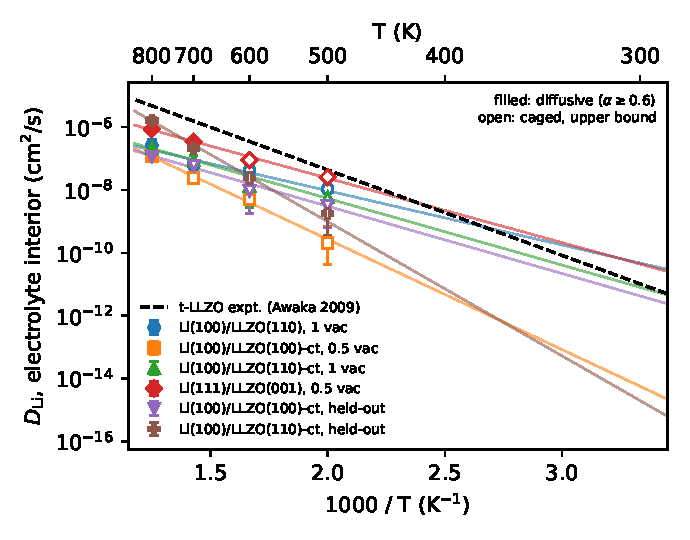
\includegraphics[width=\linewidth]{figs/fig_diffusion.pdf}
\caption{\textbf{Interior lithium transport from production molecular dynamics.}
\textbf{a}, Mean-squared displacement of interior lithium (at least 8~\AA\ below
the interface plane and 4~\AA\ above the fixed substrate) against lag time for
one replica of each interface at 500--800~K, from about 3~ns of production; the
shaded band is the 10--300~ps fit window and the dotted line has slope 1.
\textbf{b}, Arrhenius plot of the interior lithium diffusion coefficient, mean
and standard deviation over five replicas of about 3~ns each, with per-cell
Arrhenius fits. Filled symbols are diffusive points ($\alpha\geq0.6$); open
symbols are caged points that bound $D$ from above. The dashed line is the
measured conductivity of tetragonal LLZO\citep{Awaka2009} converted to a
diffusion coefficient with the Nernst--Einstein relation, with its 540~meV
activation energy. \textbf{c}, Activation energy of the interior diffusion
coefficient per cell (bars, fit uncertainty) against literature values for
tetragonal LLZO: experiment\citep{Awaka2009,Wolfenstine2012}, \emph{ab initio}
molecular dynamics\citep{Miara2013}, and simulation of the vacancy-retaining
material\citep{burov2026}. \textbf{d}, Conductivity at 300~K extrapolated from
the fits by the Nernst--Einstein relation, per cell, against the measured value
for tetragonal LLZO\citep{Awaka2009}; the band spans a factor of five either
side of experiment.}
\label{fig:msd}
\end{figure}

\begin{figure}[htbp]
\centering
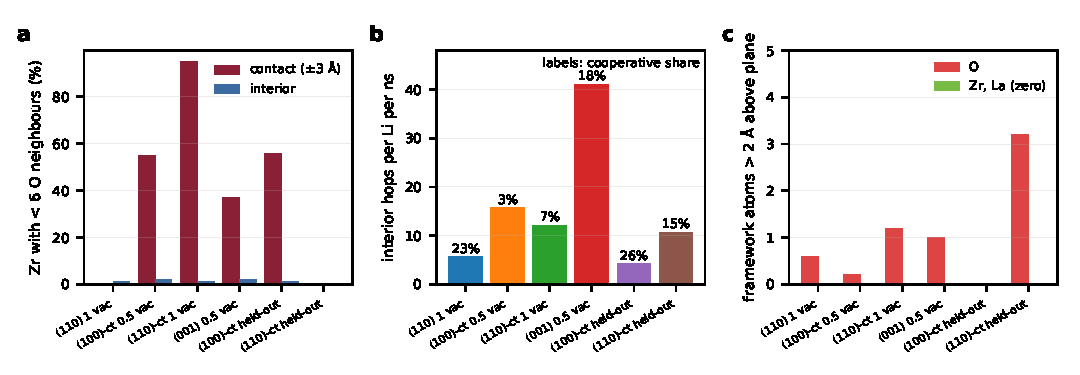
\includegraphics[width=\linewidth]{figs/fig_chemistry.pdf}
\caption{\textbf{Interface chemistry at 800~K after about 3~ns of
production.} Means over five replicas for the six interfaces of
Fig.~\ref{fig:msd}. \textbf{a}, Fraction of Zr with fewer than six O neighbours within
2.6~\AA, for Zr within $\pm3$~\AA\ of the interface plane (contact) and for Zr
in the electrolyte interior. The contact value is a property of the as-built
termination (0--96\%) and does not change between 1 and 3~ns; the interior
value is 0--2\% at every temperature. \textbf{b}, Rate of interior lithium hops,
defined as displacements above 2~\AA\ within 2~ps, per lithium per nanosecond;
labels give the share of hops in which a second lithium within 4~\AA\ hops in
the same 2~ps window. \textbf{c}, Framework atoms found more than 2~\AA\ above
the interface plane at the end of the run: 0--3 oxygen per cell and no Zr or La
in any cell. Values are transcribed from
\texttt{data/chemistry\_report\_3ns.md} and plotted by
\texttt{figs/make\_fig\_chemistry.py}.}
\label{fig:chemistry}
\end{figure}

\begin{table}[htbp]
\centering
\caption{Interface chemistry per cell at 800~K after about 3~ns of
production, means over five replicas. Undercoordinated Zr
and La are the fractions with fewer than six O within 2.6~\AA\ and fewer than
eight O within 2.9~\AA\ respectively, for atoms within $\pm3$~\AA\ of the
interface plane (contact) and in the electrolyte interior. Hops are interior
lithium displacements above 2~\AA\ within 2~ps, per lithium per nanosecond;
cooperative hops have a second lithium within 4~\AA\ hopping in the same
window. O above plane is the number of oxygen atoms more than 2~\AA\ above the
interface plane at the end of the run; Zr and La above the plane are zero in
every cell. Li--O is the first-neighbour distance and O coordination of
interior lithium. Source: \texttt{data/chemistry\_report\_3ns.md}.}
\label{tab:chemistry}
\small
\begin{tabular}{lcccccccc}
\toprule
Cell & \multicolumn{2}{c}{Zr $<6$ O (\%)} & \multicolumn{2}{c}{La $<8$ O (\%)} & Hops & Coop. & O above & Li--O (\AA) / CN \\
 & contact & interior & contact & interior & (Li$^{-1}$ns$^{-1}$) & (\%) & plane & \\
\midrule
Li(100)/LLZO(110), 1 vac            & 0  & 1 & 96 & 26 & 5.7  & 23 & 0.6 & 1.94 / 5.4 \\
Li(100)/LLZO(100)-ct, 0.5 vac       & 55 & 2 & 87 & 29 & 15.7 & 3  & 0.2 & 1.91 / 5.5 \\
Li(100)/LLZO(110)-ct, 1 vac         & 95 & 1 & 97 & 29 & 12.1 & 7  & 1.2 & 1.92 / 5.5 \\
Li(111)/LLZO(001), 0.5 vac          & 37 & 2 & 96 & 50 & 41.1 & 18 & 1.0 & 1.96 / 4.6 \\
Li(100)/LLZO(100)-ct, held-out      & 56 & 1 & 67 & 24 & 4.2  & 26 & 0.0 & 1.93 / 5.0 \\
Li(100)/LLZO(110)-ct, held-out      & 0  & 0 & 83 & 30 & 10.7 & 15 & 3.2 & 1.93 / 4.9 \\
\bottomrule
\end{tabular}
\end{table}

% ===========================================================================
\section{Discussion}
% ===========================================================================

The two components of this pipeline address complementary failures, and the
results bear on each separately.

Open-boundary labelling is validated by where the error ends up. A force RMSE of
72~meV/\AA\ is unremarkable by the standards of bulk MLIP benchmarks; what is
unusual is that it is measured against labels computed on 420--1378-atom cells
containing a single interface with two real free surfaces --- the same object
the potential is deployed on. The prevailing convention, in which a potential
is trained and validated on small periodic approximants and then applied to
large interfaces, leaves the one extrapolation that matters unmeasured. Here
there is none to make, and the error analysis shows why leaving it unmeasured
is risky: the residual concentrates by a factor of two on a free-surface layer
that bulk and sandwich training cells do not contain, so a potential trained
that way would be weakest where its own validation set is blind. What DFT-FE
contributes is therefore not a higher-capacity DFT code but boundary conditions
and a basis that make free-surface labels affordable at deployment scale, which
is the class of reference data an interface potential needs.

Latent-space acquisition is validated by whether it predicts need rather than
novelty. Uncertainty computed in the model's own latent space before labelling
predicts the force error the model turns out to have on the new structures at
$r=0.85$, measured against real DFT labels rather than a synthetic proxy and
robust to the obvious confounds. This answers the standard objection to
diversity-based selection directly, and it is convergent evidence, since the
selected structures were extreme under a criterion that ranks the pool nearly
independently. The coverage formulation also supplies something a fixed-budget
scheme cannot: a stopping criterion, which here said that a further broad
iteration would buy little. What the error localisation suggests instead is a
targeted round aimed at surface environments --- the campaign diagnosing its
own next move.

The held-out set spans the distribution the potential is deployed on, the
relevant target for a system-specific potential, and its accuracy is flat
across sub-populations: 70.0~meV/\AA\ on structures sibling to an earlier
iteration's candidate pool, 78.8~meV/\AA\ on those never selected from, and
72.1~meV/\AA\ on the independently constructed holdouts. Were familiarity
inflating the result, the sibling group would stand apart; it does not. The
improvement over the foundation model is in fact largest on the least familiar
group (54\% against 36\% on the siblings), and the final model improves on the
foundation model on 32 of the 33 structures.

\subsection*{Transfer to other systems}
\label{sec:general}

Neither component depends on this chemistry. The requirements are that a
pretrained equivariant MLIP exist for the constituent elements, to drive the
sampling dynamics and supply the latent space in which acquisition operates;
that the interface admit a slab geometry whose free surface is the physically
meaningful boundary, the generic situation for a solid--solid contact in a
battery; and that reference labels be affordable at that geometry, which the
real-space method supplies. Systems meeting these conditions include other oxide
and sulfide electrolytes in contact with lithium, and cathode$|$electrolyte
contacts, where the same interfacial-resistance questions arise and the same
periodic-sandwich compromise is currently made.

Three limitations bound the claims made here. The pipeline is demonstrated on
one interface family; whether the accuracy attained, or the number of iterations
required, carries over to chemically more complex interfaces is not established
by a single campaign. The energy channel has been flat since the third
iteration, so the campaign's gains are in forces. And the argument for open
boundaries rests on where the error sits, not on a head-to-head comparison of a
physical observable between open-boundary and periodic-sandwich constructions of
the same interface, which is the natural next test; the transport results are
likewise a consistency check against the polymorph the cells were built from,
whose room-temperature extrapolation spans four orders of magnitude in $D$.

% ===========================================================================
\section{Methods}
% ===========================================================================

\subsection{System and boundary conditions}
All structures are semi-periodic: periodic in $x$ and $y$, open in $z$, giving a
single interface with two free surfaces and no periodic-image interaction along
the surface normal\citep{dftfe,Das2022}. The condition is enforced at every stage
of the pipeline and verified on all 108 training and 33 held-out frames; the
finite $z$ extent of each cell is real-space domain padding for the
finite-element solver, not image separation.

The LLZO reference state throughout is the ordered tetragonal $I4_1/acd$
polymorph\citep{Awaka2009}. Li-metal slabs were cut from body-centred cubic Li
($a=3.51$~\AA) along (100), (110) and (111), ten atomic layers thick; LLZO
slabs were taken from prior first-principles surface studies covering
stoichiometric and non-stoichiometric terminations of several low-index
orientations\citep{Canepa2018}, and a second family of interface models, denoted
ct in Supplementary Table~S1, was adapted from the charge-transfer interfaces of
Burov \emph{et al.}\citep{Burov2024}. % VERIFY: meaning of "ct" and provenance of both slab families
For each Li/LLZO pair, in-plane supercells $(m\times n\times1)$ with
$m,n\in\{1,\dots,5\}$ were enumerated for both slabs, with in-plane mismatch
\begin{equation}
\varepsilon_i = \frac{|a_i^{\mathrm{Li}}-a_i^{\mathrm{LLZO}}|}
{\max\!\left(a_i^{\mathrm{Li}},a_i^{\mathrm{LLZO}}\right)},\qquad i\in\{a,b\},
\end{equation}
and the pair minimising $\max(\varepsilon_a,\varepsilon_b)$ was retained provided
both components were below 10\%. The LLZO supercell was held rigid and the
residual mismatch taken up by anisotropic in-plane scaling of the Li slab alone.
The Li slab was then placed above the LLZO slab at separations of 1.0--4.0~\AA\
in 0.5~\AA\ steps, each scored with the foundation model, and the lowest-energy
separation retained subject to a minimum-interatomic-distance check; the
resulting interfaces were relaxed with the foundation model (FIRE, maximum force
0.05~eV/\AA, cell fixed) before sampling. % VERIFY: gap scan and relaxation still as in thesis
Lithium-vacancy variants were generated at 0.5 and 1 vacancy per formula unit.
% [TODO] one clause on how vacancy sites were chosen.

\subsection{Reference labels}
All reference energies and forces are single-point Kohn--Sham DFT calculations
performed with DFT-FE\citep{dftfe,Das2022} using the PBE
functional\citep{pbe1996} and SPMS norm-conserving
pseudopotentials\citep{spms} for Li, La, Zr and O. The Kohn--Sham equations were
discretised on a finite-element basis of polynomial order 7, with an
automatically generated mesh of size parameter 1.2~\AA\ refined within 8.0~\AA\
of each atomic core. Self-consistency used Anderson mixing with Fermi--Dirac
smearing at an electronic temperature of 500~K and a tolerance of
$5\times10^{-5}$~Ha. Boundary conditions were periodic in $x,y$ and zero
Dirichlet in $z$ for both the wavefunctions and the electrostatic potential. No
structural relaxation was performed. Calculations ran on the OLCF Frontier
system across 64 nodes (4 AMD MI250X GPUs per node, one MPI task per GPU).

\subsection{Model architecture and fine-tuning}
The potential is a MACE equivariant message-passing
network\citep{batatia2023mace} adapted from the \texttt{mace-omat-0-medium}
foundation model pretrained on OMat24\citep{omat24}, using low-rank adaptation
(LoRA)\citep{LoRA2021} to limit catastrophic forgetting of the pretrained bulk
chemistry on a small interface dataset. For a pretrained weight matrix
$W\in\mathbb{R}^{d\times d}$ the update is constrained to a rank-$r$ subspace,
\begin{equation}
W' = W + \frac{\alpha}{r}BA,
\qquad A\in\mathbb{R}^{r\times d},\; B\in\mathbb{R}^{d\times r},\; r\ll d .
\end{equation}
Adapters are inserted in the equivariant \texttt{o3.Linear} and dense layers
using compatible irreducible representations, so the update preserves $O(3)$
equivariance. Pretrained parameters are frozen and only $(A,B)$ optimised, under
1\% of the model. Initialisation is $A\sim\mathcal{N}(0,10^{-3})$, $B=0$, so the
model begins from exactly the pretrained state; for deployment the update is
merged into $W$, giving a standard MACE model with no inference overhead.

Training minimises
\begin{equation}
L = w_E\sum_i\left(E_i-\hat{E}_i\right)^2
  + w_F\sum_i\left\|F_i-\hat{F}_i\right\|^2 ,
\end{equation}
with $w_E=1.0$, $w_F=5.0$. Hyperparameters, identical across iterations: LoRA
rank $r=5$, $\alpha=1$; batch size 8; learning rate $5\times10^{-3}$ with
\texttt{ReduceLROnPlateau} (factor 0.8, patience 50); 1500 epochs with stochastic
weight averaging from epoch 1000 at learning rate $10^{-4}$; seed 42; float32
working precision; checkpoint selection by best validation loss. Isolated-atom
reference energies (eV) were $E_0(\mathrm{Li})=-190.7590256408$,
$E_0(\mathrm{O})=-442.9888796243$, $E_0(\mathrm{Zr})=-1380.1817128081$,
$E_0(\mathrm{La})=-958.0774205521$.

\subsection{Sampling and acquisition}
Candidate configurations were generated by MLIP-driven molecular dynamics in
ASE\citep{ase} using the current iteration's model: Langevin thermostat at
1100~K with friction $10^{-3}$~fs$^{-1}$, 1~fs timestep, 50~ps per structure,
configurations recorded every 100 steps, with boundary conditions matching the
reference data. Oxide atoms deeper than $\max(0.85\,t,\,6~\text{\AA})$ below the
LLZO top surface, where $t$ is the slab thickness, were held fixed, stabilising
the far-bulk region while leaving the interface free to evolve. Frames passed a
minimum-pairwise-distance filter ($>1.2$~\AA) before entering the pool.

For each structure, a forward pass yields for each atom $i$ the rotationally
invariant ($l=0$) components of the final message-passing layer,
$\mathbf{z}_i\in\mathbb{R}^{256}$; a structure-level embedding follows by
mean-pooling, $\mathbf{Z}_S = N_S^{-1}\sum_{i=1}^{N_S}\mathbf{z}_i$, which is
L2-normalised and reduced by PCA retaining at least 95\% of variance. Selection
is farthest-point sampling seeded on the existing labelled set $\mathcal{S}$, so
that new picks complement rather than duplicate it. For each candidate $k$ in
the pool $\mathcal{P}$,
\begin{equation}
\delta_k = \min_{\mathbf{Z}_s\in\mathcal{S}}\left\|\mathbf{Z}_k-\mathbf{Z}_s\right\|_2 ,
\end{equation}
and the candidate maximising $\delta_k$ is added to $\mathcal{S}$, reducing the
coverage radius $\rho=\max_{k\in\mathcal{P}}\delta_k$, the worst-case distance
from any pool point to its nearest labelled neighbour. Selection stops when the
percentile coverage
\begin{equation}
C(d) = \frac{1}{|\mathcal{P}|}\sum_{k\in\mathcal{P}}
\mathbf{1}\!\left[\delta_k\leq d\right]
\end{equation}
reaches its target at threshold $d$ --- a stopping rule set by the pool's own
geometry rather than a fixed per-round budget. For the analysis of
Section~\ref{sec:uq}, a Gaussian-process posterior variance was computed in the
same feature space conditioned on the pre-round training set.

\subsection{Evaluation}
The held-out set comprises 33 structures, disjoint from training: 21 are
siblings of an earlier iteration's candidate pool, 8 come from pools never
selected from, and 4 were constructed independently of any selection round.
Candidate test entries duplicating training configurations were identified by
model prediction and removed (Supplementary Note~3). Structures above the trained
vacancy range are excluded from the primary metric and reported separately.

Force error is component-wise throughout:
$\mathrm{RMSE}=\sqrt{\langle(F_{\mathrm{pred}}-F_{\mathrm{ref}})^2\rangle}$ over
all atoms and all three Cartesian components, in meV/\AA; multiply by $\sqrt{3}$
for the RMS of per-atom error vectors. Energy error is
$|E_{\mathrm{pred}}-E_{\mathrm{ref}}|/N$ in meV/atom. Paired model comparisons use
the Wilcoxon signed-rank test over structures. Evaluation is performed in
float32, matching training; at the absolute energies of these cells this limits
the resolution of the energy metric to $\sim$0.1~meV/atom, while force errors
reproduce exactly.

\subsection{Transport simulations and analysis}
Production trajectories were run with the NVIDIA ALCHEMI
toolkit\citep{alchemi} using cuEquivariance kernels in float32, one or two
interfaces per A100 GPU across 100 nodes of the PARAM Rudra system. Each of the
six interfaces was simulated at 500, 600, 700 and 800~K with five replicas
differing in initial velocities, under a Nos\'e--Hoover
thermostat\citep{Nose1984,Hoover1985} (coupling time 100~fs) with a 2~fs timestep
and the open-$z$ boundary conditions of the reference data; configurations were
recorded every 2~ps, and each replica ran for 2.95--3.1~ns. The oxide substrate
is fixed as in the sampling runs, and in addition the outermost
$\max(0.15\,t_{\mathrm{Li}},4~\text{\AA})$ of the metal slab, where
$t_{\mathrm{Li}}$ is its thickness, is held fixed as a stand-in for the bulk
electrode: without it the free surface of the lattice-matched, strained metal
slab disorders the whole slab at every temperature studied. Lithium inside the
electrolyte is never constrained. The thermostat target is scaled by the mobile
fraction of atoms so that the mobile population is at the nominal temperature.
Two small numerical artefacts of the production runs, a slow drift of the
fixed atoms and a frame gap at one restart boundary, are characterised in
Supplementary Note~6; both are estimated to bias $D$ by less than the replica
scatter.

The first 100~ps of each trajectory are discarded. Interior lithium is defined
at that time as the atoms at least 8~\AA\ below the interface plane --- the 98th
percentile of La/Zr/O height in each frame --- and at least 4~\AA\ above the
fixed substrate, restricted to atoms that never enter the metal. Their
mean-squared displacement is accumulated over all time origins in unwrapped
fractional coordinates, without centre-of-mass correction, and $D$ is the
Einstein slope over lags of 10--300~ps divided by 6, a window chosen because
the 500--600~K curves are not linear at longer lags; a 50--1000~ps window
leaves every conclusion unchanged (Supplementary Note~7), and the in-plane
coefficient agrees with the total within the replica scatter. The anomalous-diffusion exponent
$\alpha$ is the log--log slope over the same window, the effective number of
hops is the total mean-squared displacement divided by the squared hop length of
3~\AA\ (ref.~\citenum{He2018}), and uncertainties are standard deviations over
the five replicas. Activation energies are from a weighted least-squares
Arrhenius fit to the four temperatures; conductivities follow from the
Nernst--Einstein relation with the interior lithium density and a Haven ratio
of one. Interface crossings are counted against a $\pm1.5$~\AA\ hysteresis band
about the interface plane, following ref.~\citenum{burov2026}. For the
interface chemistry, Zr and La coordination numbers count oxygen within 2.6 and
2.9~\AA\ respectively, framework atoms are counted as displaced when more than
2~\AA\ above the interface plane, an interior hop is a lithium displacement
above 2~\AA\ within 2~ps, and a hop is cooperative when a second lithium within
4~\AA\ hops in the same window; all are averaged over the five replicas.

\subsection*{Code availability}
[TODO: repository and archive DOI for training, acquisition, evaluation and
MD/analysis scripts.]

\subsection*{Data availability}
[TODO: repository and persistent identifier (DOI) for the DFT-FE reference
labels, training and test structure files, and trained model checkpoints.]

\section*{Acknowledgements}
[TODO: named acknowledgements.] Model training, inference and sampling
molecular dynamics were carried out on the KIAC Mahamathi cluster (NVIDIA H200
and A5000 GPUs); production molecular dynamics on the PARAM Rudra system (NVIDIA
A100) of the National Supercomputing Mission; DFT-FE single-point calculations
on the OLCF Frontier supercomputer.

\section*{Competing Interests}
The authors declare no competing interests.

\section*{Contributions}
M.D. designed and ran the active-learning campaign, model training, evaluation
and production dynamics, and wrote the manuscript. [TODO: R.B., K.R., G.P.D.]
P.M. supervised the project and is the guarantor of this work.

\section*{Funding}
[TODO: grant/funding-body statement, or ``Not applicable''.]

\section*{Supplementary Information}
Supplementary Information accompanies this paper at the \emph{npj
Computational Materials} website.

% ===========================================================================
% REFERENCES  (replace with pasted .bbl before submission)
% ===========================================================================
\begin{thebibliography}{99}

\bibitem{batatia2023mace}
Batatia, I., Kov\'acs, D. P., Simm, G. N. C., Ortner, C. \& Cs\'anyi, G. MACE:
Higher order equivariant message passing neural networks for fast and accurate
force fields. \emph{Adv. Neural Inf. Process. Syst.} \textbf{35} (2022).

\bibitem{batatia2023foundation}
Batatia, I. \emph{et al.} A foundation model for atomistic materials chemistry.
Preprint at https://arxiv.org/abs/2401.00096 (2023).

\bibitem{omat24}
Barroso-Luque, L. \emph{et al.} Open Materials 2024 (OMat24) inorganic materials
dataset and models. Preprint at https://arxiv.org/abs/2410.12771 (2024).

\bibitem{dftfe}
Motamarri, P. \emph{et al.} DFT-FE -- A massively parallel adaptive
finite-element code for large-scale density functional theory calculations.
\emph{Comput. Phys. Commun.} \textbf{246}, 106853 (2020).

\bibitem{Das2022}
Das, S., Motamarri, P., Subramanian, V., Rogers, D. M. \& Gavini, V. DFT-FE 1.0:
A massively parallel hybrid CPU-GPU density functional theory code using
finite-element discretization. \emph{Comput. Phys. Commun.} \textbf{280},
108473 (2022).

\bibitem{vargaumbrich2026}
Varga-Umbrich, E. \emph{et al.} Pretrained model representations as acquisition
signals for active learning of MLIPs. In \emph{Proc. 43rd International
Conference on Machine Learning (ICML 2026)}. Preprint at
https://arxiv.org/abs/2605.03964.

\bibitem{Iwasaki2022}
Iwasaki, R. \emph{et al.} Density functional theory studies on Li metal
electrode/garnet-type Li$_7$La$_3$Zr$_2$O$_{12}$ solid electrolyte interfaces
for application in all-solid-state batteries. \emph{Phys. Status Solidi B}
\textbf{259}, 2100546 (2022).

\bibitem{Burov2024}
Burov, A. S., Boev, A. O., Abakumov, A. M. \& Aksyonov, D. A. Mechanism of
Li$^+$ charge transfer at Li/Li$_7$La$_3$Zr$_2$O$_{12}$ interfaces: a density
functional theory study. \emph{Phys. Rev. B} \textbf{109}, 045305 (2024).

\bibitem{Iwasaki2024}
Iwasaki, R., Tanibata, N., Takeda, H. \& Nakayama, M.
Universal-neural-network-potential molecular dynamics for lithium metal and
garnet-type solid electrolyte interface. \emph{Commun. Mater.} \textbf{5}, 148
(2024).

\bibitem{He2018}
He, X., Zhu, Y., Epstein, A. \& Mo, Y. Statistical variances of diffusional
properties from ab initio molecular dynamics simulations. \emph{npj Comput.
Mater.} \textbf{4}, 18 (2018).

\bibitem{Awaka2009}
Awaka, J., Kijima, N., Hayakawa, H. \& Akimoto, J. Synthesis and structure
analysis of tetragonal Li$_7$La$_3$Zr$_2$O$_{12}$ with the garnet-related type
structure. \emph{J. Solid State Chem.} \textbf{182}, 2046--2052 (2009).

\bibitem{Wolfenstine2012}
Wolfenstine, J., Rangasamy, E., Allen, J. L. \& Sakamoto, J. High conductivity
of dense tetragonal Li$_7$La$_3$Zr$_2$O$_{12}$. \emph{J. Power Sources}
\textbf{208}, 193--196 (2012).
% VERIFY: the 0.41 eV value quoted from this reference.

\bibitem{Miara2013}
Miara, L. J. \emph{et al.} Effect of Rb and Ta doping on the ionic conductivity
and stability of the garnet
Li$_{7+2x-y}$(La$_{3-x}$Rb$_x$)(Zr$_{2-y}$Ta$_y$)O$_{12}$ superionic conductor:
a first principles investigation. \emph{Chem. Mater.} \textbf{25}, 3048--3055
(2013).
% VERIFY: the 0.43 eV AIMD value for the undoped tetragonal composition.

\bibitem{burov2026}
Burov, A. S., Abakumov, A. M. \& Aksyonov, D. A. Machine learning assisted
molecular dynamics of charge-transfer mechanisms at Li/Ga-doped
Li$_7$La$_3$Zr$_2$O$_{12}$ (LLZO) interfaces. Preprint at
https://arxiv.org/abs/2606.07772 (2026).

\bibitem{Krauskopf2019}
Krauskopf, T. \emph{et al.} Toward a fundamental understanding of the lithium
metal anode in solid-state batteries --- an electrochemo-mechanical study on
the garnet-type solid electrolyte Li$_{6.25}$Al$_{0.25}$La$_3$Zr$_2$O$_{12}$.
\emph{ACS Appl. Mater. Interfaces} \textbf{11}, 14463--14477 (2019).

\bibitem{Murugan2007}
Murugan, R., Thangadurai, V. \& Weppner, W. Fast lithium ion conduction in
garnet-type Li$_7$La$_3$Zr$_2$O$_{12}$. \emph{Angew. Chem. Int. Ed.}
\textbf{46}, 7778--7781 (2007).

\bibitem{Canepa2018}
Canepa, P. \emph{et al.} Particle morphology and lithium segregation to surfaces
of the Li$_7$La$_3$Zr$_2$O$_{12}$ solid electrolyte. \emph{Chem. Mater.}
\textbf{30}, 3019--3027 (2018).

\bibitem{pbe1996}
Perdew, J. P., Burke, K. \& Ernzerhof, M. Generalized gradient approximation
made simple. \emph{Phys. Rev. Lett.} \textbf{77}, 3865--3868 (1996).

\bibitem{spms}
Shojaei, M. F., Pask, J. E., Medford, A. J. \& Suryanarayana, P. Soft and
transferable pseudopotentials from multi-objective optimization.
\emph{Comput. Phys. Commun.} \textbf{283}, 108594 (2023).

\bibitem{LoRA2021}
Hu, E. J. \emph{et al.} LoRA: low-rank adaptation of large language models. In
\emph{Proc. International Conference on Learning Representations (ICLR 2022)}.
Preprint at https://arxiv.org/abs/2106.09685.

\bibitem{ase}
Larsen, A. H. \emph{et al.} The atomic simulation environment --- a Python
library for working with atoms. \emph{J. Phys.: Condens. Matter} \textbf{29},
273002 (2017).

\bibitem{alchemi}
NVIDIA. ALCHEMI Toolkit. https://github.com/NVIDIA/nvalchemi-toolkit (2026).
% [TODO] pin the version used on PARAM Rudra.

\bibitem{Nose1984}
Nos\'e, S. A unified formulation of the constant temperature molecular dynamics
methods. \emph{J. Chem. Phys.} \textbf{81}, 511--519 (1984).

\bibitem{Hoover1985}
Hoover, W. G. Canonical dynamics: equilibrium phase-space distributions.
\emph{Phys. Rev. A} \textbf{31}, 1695--1697 (1985).

\end{thebibliography}

\end{document}
